This project attempts to deliver on a haptics focused terrain editing experience first and foremost. The overaching approach was to first establish a reliable coupling via a virtual proxy to Unity's physics system, and then create a proof of concept terrain editing tool which is driven by the aforementioned virtual proxy.

The three fundamental questions we had were as follows:

\begin{enumerate}
    \item How would we design a generic virtual coupling between Unity's physics engine and the Haply's force feedback mechanisms?
    \item How would we detect and render textures in realtime?
    \item How would we design the tool itself, with the main mode of interaction being through the Haply?
\end{enumerate}

\subsection{How would we design a generic virtual coupling between Unity's physics engine and the Haply's force feedback mechanisms?}

We initially employed the Unity template obtained from the Haply GitLab repository as the foundation for our implementation. However, upon closer examination, it became evident that the forces applied were hardcoded, prompting us to adopt a \textit{PD controller} model facilitated by a virtual proxy (\textit{See \ref*{fig:virtual-coupling}}), as elaborated below.

In our implementation, we utilized Unity game objects, specifically employing one designated as the "\textbf{End Effector Actual}" to track the ideal positional data of the Haply, and another marked as the "\textbf{End Effector Representation}" equipped with a built-in sphere collider. This was to allow it to interact with Unity's physics engine. Subsequently, we established a \textit{PD controller} relationship between these two entities. The underlying operational logic mandated the "\textbf{End Effector Representation}" to consistently attempt to minimize the euclidean distance between itself and the "\textbf{End Effector Actual}". This behavior was governed primarily by the proportional component of the \textit{PD controller}, supplemented by the derivative component to offer additional smoothing (\textit{See \ref*{fig:virtual-coupling-a}}). In instances where the "\textbf{Representation}" detected any physical collisions, it directed the Haply to exert a force in the direction of the "\textbf{Representation}" from the "\textbf{Actual}" (\textit{See \ref*{fig:virtual-coupling-b}}). This would happen in parallel to the distance minimization attempts of the "\textbf{Representation}". Consequently, this establishment facilitated an adaptable virtual coupling mechanism, subject to the influence of Unity's physics engine via the intermediary proxy.

\begin{figure}[htbp]
    \centering
    \begin{subfigure}[b]{0.4\textwidth}
        \centering
        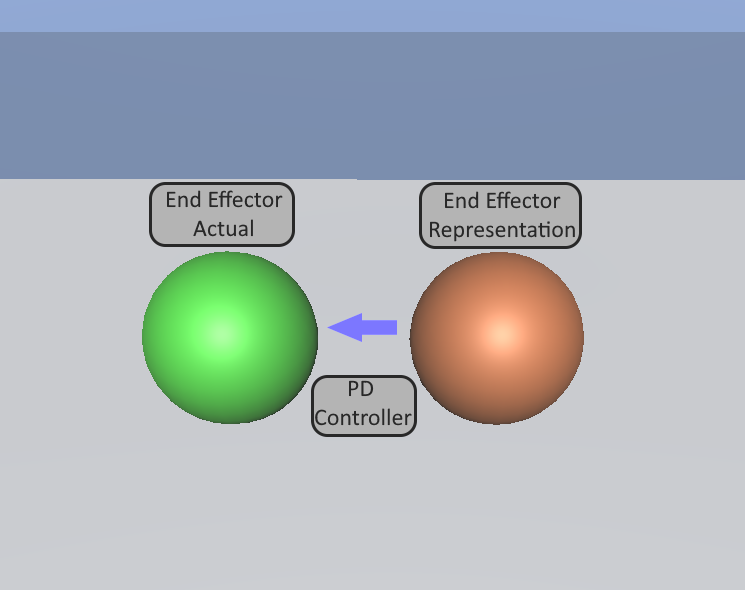
\includegraphics[width=\textwidth]{images/approach-virtual-coupling-a.png}
        \caption{PD controller moves Representation to Actual if there is no obstruction}
        \label{fig:virtual-coupling-a}
    \end{subfigure}
    \quad
    \quad
    \begin{subfigure}[b]{0.4\textwidth}
        \centering
        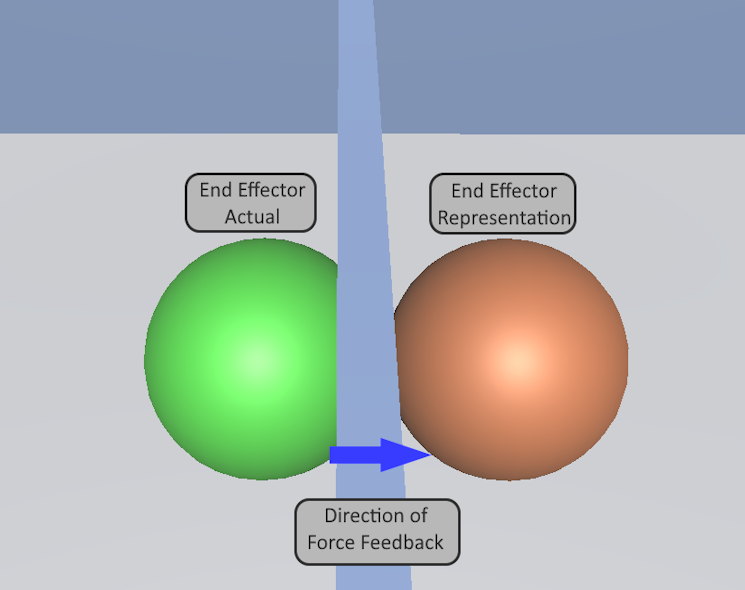
\includegraphics[width=\textwidth]{images/approach-virtual-coupling-b.png}
        \caption{Force Feedback Rendered if physics collision is detected}
        \label{fig:virtual-coupling-b}
    \end{subfigure}
    \caption{Virtual Coupling between Representation and Actual End Effector}
    \label{fig:virtual-coupling}
\end{figure}

Notably, while the direction vector was three-dimensional, only the X and Z components of this vector were translated to the Haply to render force feedback. The selected axes were simply an artifact our design decision for editing on a terrain lying in the X-Z plane.

\subsection{How would we detect and render textures in realtime?}

Lorem Ipsum

\subsection{How would we design the tool itself, with the main mode of interaction being through the Haply?}

Lorem Ipsum set dolor 
